\section{Práticas para o Desenvolvimento de Software de Pesquisa Sustentável} \label{section:practices}

Projetos de software bem organizados adotam um modelo de desenvolvimento que resulta em código de alta qualidade que se adapta rapidamente a diferentes situações. Várias \textit{práticas} estabelecidas e usadas pelas comunidades de software livre são reconhecidas como contribuições importantes para a manutenção de \RSw de alta qualidade.
%
Nesta seção, apresentamos dezesseis boas práticas para uso em projetos de \RS, descritas e ilustradas no contexto de projetos hospedados no GitHub.
Parte do jargão técnico usado pelo GitHub não foi traduzido e alguns termos não foram definidos. Termos e suas definições podem ser encontrados no \textit{Glossário do GitHub}\footnote{\url{https://docs.github.com/en/get-started/quickstart/github-glossary}}.

\subsection{Práticas Básicas}

\subsection*{P1. Hospedagem do projeto} 

É recomendável hospedar e compartilhar o \RSw em um repositório público, exceto se houver questões de confidencialidade ou estratégicas relacionadas ao projeto de pesquisa (por exemplo, software implementa um algoritmo original, ainda não compartilhado amplamente com a comunidade científica). 
A hospedagem em repositório público pode ser estendida para todos os ativos da pesquisa, por exemplo, dados, fluxos de trabalho e relatórios.

A \textit{hospedagem pública do software} é fundamental para promover a reprodutibilidade, evitar a redundância (por exemplo, cópias do software em diversos repositórios locais), 
e estimular o compartilhamento entre pares da comunidade acadêmica.
%
A hospedagem pública do software e o acesso aos dados e fluxos de trabalho, permitem que os resultados da pesquisa possam ser verificados, replicados, e reproduzidos, fortalecendo a confiabilidade e a transparência dos estudos. 
%
Além disso, o \RSw hospedado torna-se localizável e acessível, facilitando seu uso ou reuso.
Se o código for aberto, outros pesquisadores podem se beneficiar dele, evitando o retrabalho e construindo sobre uma base já estabelecida. Isso promove a colaboração, a troca de conhecimentos e a aceleração do progresso científico.

\noindent \textbf{Exemplo.}
O \RSw \texttt{flosssearch} estava hospedado em uma pasta local no computador de um pesquisador. 
Por segurança, o pesquisador realizava backup manual periodicamente. 
Ao finalizar a implementação da primeira funcionalidade do software, o pesquisador decidiu que o projeto precisava ser hospedado adequadamente e compartilhado com outros membros do grupo de pesquisa.
%Uma organização foi criada no GitHub e o
O software \texttt{flosssearch} foi colocado em um repositório público no GitHub, uma plataforma baseada na web onde os usuários podem hospedar repositórios, compartilhar e promover a colaboração em projetos de software.
%
O repositório foi compartilhado com dois pesquisadores do grupo.
% Mensagem de \textit{commit}: \textit{v 0.0.1 - Versionando}.

Ao ser hospedado no GitHub, o software recebeu uma URL, um nome oficial e a sua identidade foi definida, de forma clara e única. 
O nome oficial público atribuído ao \RSw é \texttt{flosssearch}.
Além disso, o software \texttt{flosssearch} passou a contar com um serviço de backup, considerando que os arquivos do projeto e todo o seu histórico são armazenados no servidor remoto e nos repositórios locais dos pesquisadores.

\subsection*{P2. Controle de versão} 

Controle de versão é a prática de rastrear e gerenciar alterações no código de um software. 
Os sistemas de controle de versão são ferramentas que
permitem que várias versões do mesmo \RSw sejam mantidas e, possivelmente, referenciadas por experimentos de pesquisa e artigos científicos. 
Um sistema de controle de versão também permite o acompanhamento das atividades realizadas, fornece um registro das alterações e permite que desenvolvedores e usuários do \RSw acompanhem o seu desenvolvimento e evolução, tornando a pesquisa mais aberta
e reprodutível. 
Ao usar o controle de versão, o pesquisador nunca perde as versões anteriores do \RS, e erros podem ser revertidos.
Adicionalmente, o versionamento do software também promove a colaboração entre pesquisadores.

%It is highly recommended to start using version control on day one of the project.

\noindent \textbf{Exemplo.}
A plataforma GitHub utiliza o Git\footnote{\url{https://git-scm.com}}, um sistema de controle de versão distribuído gratuito e de código aberto. 
Ao ser colocado no GitHub, com um nome e repositório associado, 
o \RSw \texttt{flosssearch} recebeu suporte para controle de versão distribuído. 
%... versão  \textit{v 0.0.1 - Versionando projeto} ... 4 anos atrás.

\subsection*{P3. Licenças de Software} 
% Nesta seção apresentaremos aspectos de Licenças de Software relevantes para o Software de Pesquisa e para alavancar a Ciência Aberta. 

%Alguns dos tópicos: \textit{Open Source Software}, \textit{Open Source Initiative}\footnote{\url{https://opensource.org/licenses}}, licenças populares e amplamente utilizadas ou com comunidades fortes, tais como a GNU General Public License (GPL) ou a Mozilla Public License 2.0.

% Olhar no GitHub o projeto ChooseaLicense

A licença de software escolhida é essencial para o \RSw disponível publicamente. O financiamento do projeto pode terminar após um certo período, e os mantenedores podem terminar suas pesquisas ou mudar de área de interesse. Assim, para garantir a disponibilidade contínua do projeto, os desenvolvedores precisam chegar a um acordo formal, ou seja, uma licença de software em que os termos de uso sejam explícitos.

Recomenda-se que projetos de \RSw de código aberto sejam lançados sob uma licença compatível com a GNU General Public License - GPL\footnote{\url{https://www.gnu.org/licenses/gpl-3.0.html}},
a licença OSS mais popular e amplamente utilizada.
Outras licenças de software de código aberto e suas descrições podem ser encontradas no site da Open Source Initiative (OSI)\footnote{\url{https://opensource.org/licenses/}}.

O GitHub permite que o usuário escolha uma licença de software para o seu repositório e cria automaticamente o arquivo \textit{LICENSE} com uma cópia da licença escolhida.
Entretanto, apenas colocar uma cópia da licença em um arquivo em seu repositório não declara explicitamente que o código no  repositório pode ser usado sob tal licença. 
Sem uma declaração explícita, não fica claro se as permissões da licença se aplicam a qualquer arquivo fonte no repositório.

A Figura~\ref{fig:warranty} mostra um aviso que o desenvolvedor deve incluir no início de cada arquivo fonte para declarar a licença e a exclusão da garantia. Cada arquivo deve ter pelo menos a linha ``copyright'' e indicação sobre local onde o aviso completo pode ser encontrado.
%
A falta de uma licença claramente definida pode gerar incerteza legal e dificultar a contribuição e o compartilhamento do software, já que os colaboradores podem ficar inseguros sobre seus direitos e obrigações, o que pode limitar a adoção e colaboração.

\renewenvironment{quote}
  {\small\list{}{\rightmargin=1cm \leftmargin=1cm}%
   \item\relax}
  {\endlist}
\begin{figure}[htb]
    \centering
\begin{quote}
\textit{<one line to give the program's name and a brief idea of what it does.>}
    
Copyright (C) \textit{<year>}  \textit{<name of author>}

This program is free software: you can redistribute it and/or modify it under the terms of the GNU General Public License as published by the Free Software Foundation, either version 3 of the License, or (at your option) any later version.

This program is distributed in the hope that it will be useful, but WITHOUT ANY WARRANTY; without even the implied warranty of MERCHANTABILITY or FITNESS FOR A PARTICULAR PURPOSE. See the
GNU General Public License for more details.
You should have received a copy of the GNU General Public License along with this program.  If not, see <https://www.gnu.org/licenses/>.
\end{quote}
\caption{Declaração explícita sobre uso de licença GPL e exclusão da garantia.} \label{fig:warranty}
\end{figure}

\noindent\textbf{Exemplo.}
Ao ser colocado em um repositório público no GitHub, 
o \RSw \texttt{flosssearch} tornou-se visível, acessível e utilizável por terceiros, sendo necessária a escolha de uma licença de código aberto. Os pesquisadores escolheram a licença GNU GPL 3.0. 
Além do arquivo LICENSE, os arquivos com código-fonte do projeto possuem uma breve descrição sobre o seu propósito, a linha ``copyright'' e indicação sobre a licença de software escolhida e onde o texto completo pode ser encontrado (Figura~\ref{fig:license:moara}).

%Apesar da linguagem PHP possuir um framework para automação de testes, o \textit{PHPUnit}, o software \texttt{flosssearch} não possui testes automatizados. 
%A falta de testes pode dissuadir desenvolvedores de consertar, estender ou melhorar o \RS, e outros pesquisadores de usá-lo. 

\renewenvironment{quote}
  {\small\list{}{\rightmargin=1cm \leftmargin=1cm}%
   \item\relax}
  {\endlist}
\begin{figure}[htb]
\centering
\begin{quote}
\texttt{flossearch} is a web application designed to support instructors and students in selecting OSS projects for Software Engineering Education.

Copyright (C) \textit{2021}  \textit{Moara Brito}

This program is free software: you can redistribute it and/or modify it under the terms of the GNU General Public License 3.0 <https://www.gnu.org/licenses/>.
\end{quote}
\caption{Declaração sobre uso de licença GPL para inclusão nos arquivos do \texttt{flosssearch}.} \label{fig:license:moara}
\end{figure}

% O arquivo README.md ...

\subsection*{P4. Registro de Software}

O \RSw deve ser publicado formalmente para satisfazer os princípios FAIR, promover a sustentabilidade de software e permitir a citação de software. Os repositórios de publicação dão suporte ao registro do software e fornecem versões de software publicadas com identificadores únicos e persistentes, como um DOI.

Há várias formas de associar um DOI a um repositório GitHub. 
Zenodo\footnote{\url{https://zenodo.org}} e Figshare\footnote{\url{https://figshare.com}} 
podem ser utilizados para fazer o registro do DOI e arquivar versões especificas do software. 
%
Há também o projeto {\em The Research Software Directory}\footnote{\url{https://research-software-directory.org}} desenhado para centralizar metadados de software de pesquisa e mostrar os seus impactos na pesquisa e na sociedade, estimulando o reuso de software e encorajando a citação de maneira apropriada para garantir que pesquisadores e engenheiros de \RSw  recebam créditos por seus trabalhos. 

\noindent \textbf{Exemplo.}
O \RSw \texttt{Parcels}\footnote{\url{https://github.com/OceanParcels/parcels}} (\textbf{P}robably \textbf{A} \textbf{R}eally \textbf{C}omputationally \textbf{E}fficient \textbf{L}agrangian \textbf{S}imulator) é um conjunto de classes e métodos em Python para criar simulações de rastreamento de partículas, como plâncton, plástico e peixes. 
O \texttt{Parcels} está registrado no Research Software Directory\footnote{\url{https://research-software-directory.org/software/parcels}}.


%O Zenodo se integra ao GitHub para arquivar o software e fornecer um DOI quando os desenvolvedores fizerem um lançamento formal no GitHub.

%\noindent \textbf{\texttt{seed.select}}.

% Movi pra parte de Avaliação
%\noindent \textbf{\texttt{Software MoSyn}}.
%O repositório não menciona se há um DOI associado a ele e não encontramos referência ao software no Zenodo.


%---------------------------------------------%
\subsection{Organização do Projeto}

O suporte à reprodutibilidade na pesquisa que utiliza um \RSw requer que seus artefatos estejam bem organizados em um repositório aberto. 

\begin{figure}[htb]
    \centering
    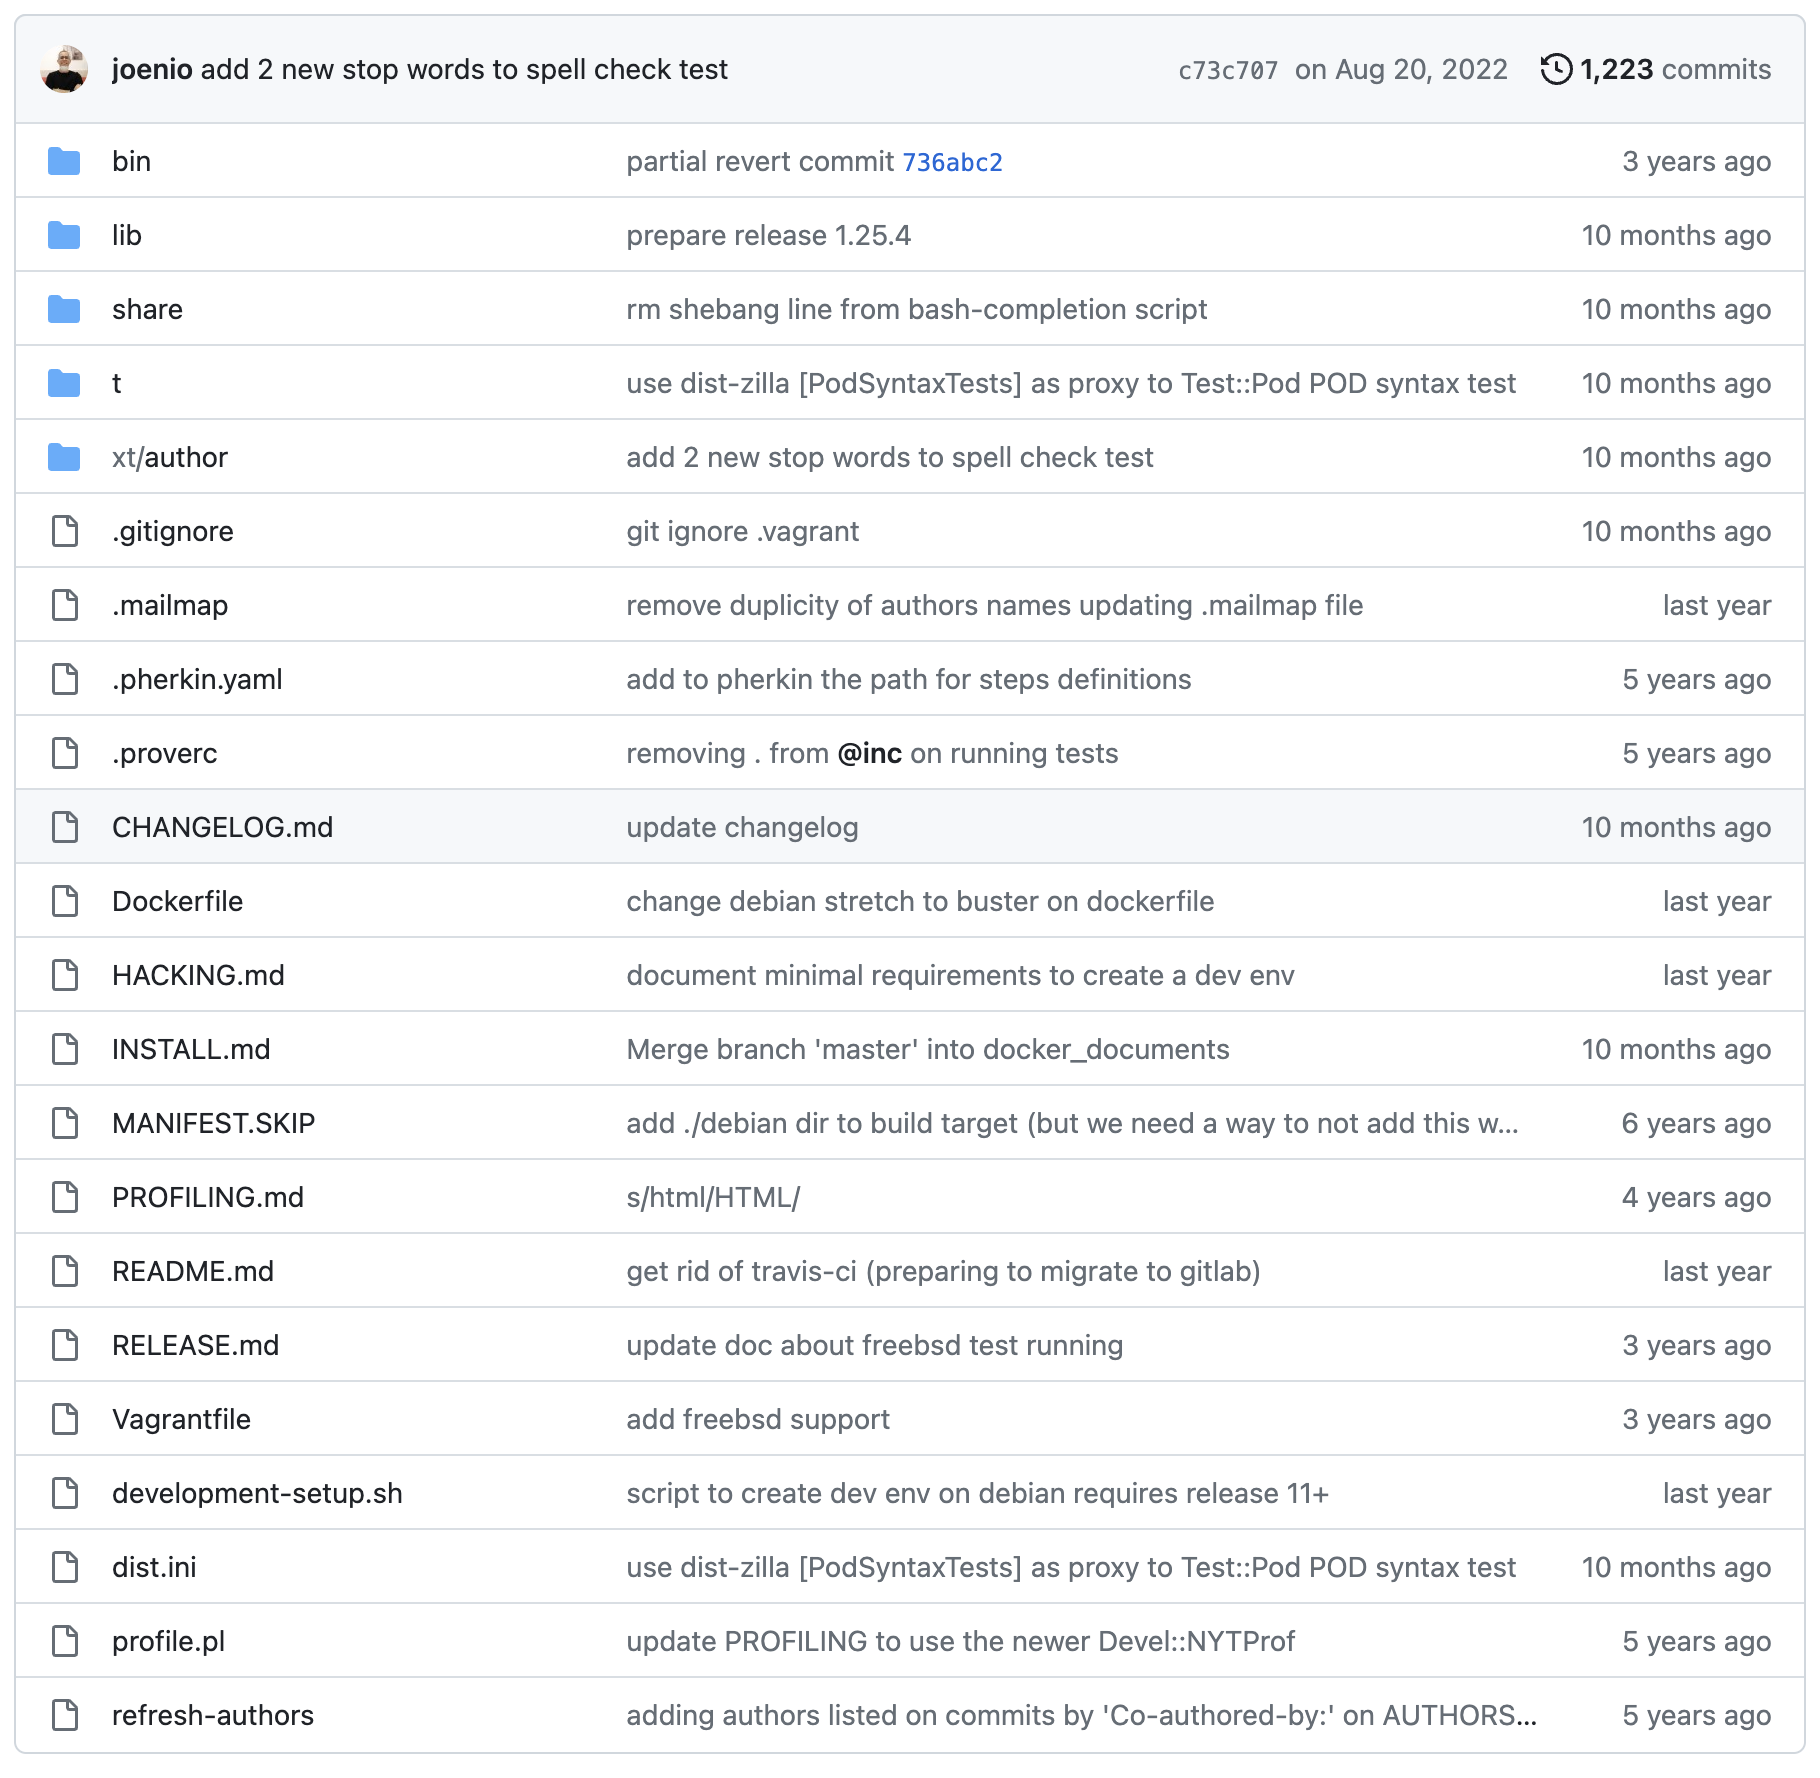
\includegraphics[scale=0.45]{JAI 2023/figures/analizo-estrutura.png}
    \caption{Estrutura de arquivos da ferramenta \texttt{Analizo}.}
    \label{fig:estrutura:analizo}
\end{figure}

\subsection*{P5. Estrutura} 

É importante ter uma estrutura de arquivos que comunica a finalidade dos elementos dentro de um \RS, separando os interesses em uma hierarquia de pastas e usando nomes auto-explicativos, facilitando a compreensão de todos que tenham interesse revisitar, revisar e desenvolver o software.

\noindent\textbf{Exemplo.} A Figura~\ref{fig:estrutura:analizo} apresenta a estrutura de arquivos da ferramenta de análise estática \texttt{Analizo}\footnote{\url{https://github.com/analizo/analizo}}\cite{analizo2010}, desenvolvida como \RSw no contexto de uma pesquisa de doutorado. Pode-se observar que há pastas e arquivos com nomes auto-explicativos, por exemplo, \textit{bin}, \textit{lib} e \textit{share}, INSTALL.md, README.md.

\subsection*{P6. Padronização} 
% Use standards

%O uso de formatos de dados e interfaces padronizados facilita a integração com outros sistemas e desencoraja a dependência de fornecedores específicos. 

A padronização e o uso de protocolos de comunicação entre sistemas tem uma grande importância no software de pesquisa. A partir da adoção de padrões e protocolos bem definidos, os diferentes sistemas podem interagir de forma consistente, facilitando a integração e desencoraja a dependência de fornecedores específicos. Além disso, a padronização simplifica a interoperabilidade e a reutilização de componentes de software, permitindo que os pesquisadores desenvolvam seus trabalhos sobre trabalhos existentes e tornem mais rápido o desenvolvimento de novas soluções.

\noindent\textbf{Exemplo.} O software \texttt{MoSyn} é um \RSw que se preocupa com padronização pois depende de um software proprietário, o  MATLAB\footnote{\url{https://www.mathworks.com/products/matlab.html}}. A Seção~\ref{section:casesstudy:mosyn} apresenta uma avaliação do \texttt{MoSyn} com base nas práticas para o desenvolvimento adotadas.

%---- Qualidade -----%
% Geral: Higher quality software has fewer defects, better security, and better performance, which leads to happier users who can work more effectively.

\subsection*{P7. Documentação} 

A documentação frequente e contínua é uma prática recomendada para manter guias do usuário, manuais e outros documentos relevantes atualizados em relação à versão mais recente do software, facilitando o entendimento e colaboração.
Para o \RS, a documentação é um pré-requisito fundamental para reuso e reprodução de estudos~\cite{chue_hong_fair_2022}.
%
\cite{herman:2022} analisaram o estado-da-prática sobre documentação de \RS. Eles reportaram que, ainda que alguns guias com boas práticas científicas valorizem e recomendem a prática de documentar explicitamente~\cite{deutsche_forschungsgemeinschaft_2022_6472827},  
a documentação do \RSw ainda é considerada inadequada~\cite{wilson2017good, chue_hong_fair_2022}.

%- Como manter a documentação atualizada?

%Developers usually change code, correcting bugs, adding new functionalities but not do any modification in documentation, this turn it outdated. However the documentation is useful only if it's up to date. 
%
%Before you submit your change, write the documentation related to it.
%Core developers should require this from the contributors.

A documentação de um projeto só é útil se está atualizada. Por isso, uma questão importante em um projeto de software é a sincronização entre o desenvolvimento do software e a documentação dele, garantindo que a documentação representa a versão mais atualizada do software. 
Para conseguir essa sincronização é essencial integrar o processo de atualização da documentação no ciclo de desenvolvimento do software. Além disso, é possível automatizar a geração de documentação a partir de comentários no código-fonte, reduzindo o esforço necessário para manter a documentação atualizada.

Em geral, geradores de documentação são usado para interfaces de programação de aplicativos (APIs), destinadas a um público de desenvolvedores. 
\textit{Doxygen}\footnote{\url{https://www.doxygen.nl}} é uma ferramenta que extrai documentação a partir do código-fonte e de outros arquivos e gera uma versão em formato estruturado, como HTML, PDF ou LaTeX. 
%
Doxygen é a ferramenta padrão de fato para gerar documentação para C++, mas também suporta outras linguagens de programação populares como C, Objective-C, C\#, PHP, Java e Python.

Uma documentação precisa ser clara e considerar os diferentes interessados no \RS. A documentação precisa atender às necessidades específicas de cada grupo, usando linguagem e terminologia que ajudem cada público a compreender e utilizar as informações de maneira eficaz.

%- Como escrever documentação clara e útil para desenvolvedores?
%Para escrever documentação clara e útil para desenvolvedores
A \textit{documentação para desenvolvedores} deve abordar aspectos técnicos, como arquitetura, APIs, dependências e configurações, incluindo descrições detalhadas de como utilizar as funcionalidades do software. É importante que sejam fornecidas orientações passo-a-passo sobre instalação, configuração, execução e dependências necessárias para o ambiente de desenvolvimento do software. 
Para facilitar a contribuição, é essencial descrever conceitos fundamentais, padrões de codificação e boas práticas de desenvolvimento.
Testes de software também oferecem uma forma de documentar a funcionalidade do software por meio da
qual desenvolvedores podem ter uma visão mais detalhada sobre o funcionamento interno do software e integração com outros sistemas.

%- Como escrever documentação útil para não desenvolvedores, outros pesquisadores?
Na \textit{documentação para pesquisadores} que não são desenvolvedores, deve-se utilizar uma linguagem acessível, evitando jargões técnicos e explicando conceitos de forma simples e compreensível. 
A descrição da utilização deve destacar as  funcionalidades e benefícios do software. 
Para facilitar o uso, podem ser apresentados exemplos práticos de como o \RSw pode ser aplicado em diferentes cenários e incluir uma seção de perguntas frequentes para responder às dúvidas mais comuns dos usuários. Dessa forma, a documentação para os pesquisadores que não são desenvolvedores pode ajudá-los a entender como utilizar o software de forma prática para atingir seus objetivos de pesquisa, sem detalhes técnicos desnecessários.

Para todos os tipos de usuários,
recomenda-se que, ao publicar o \RS, o desenvolvedor  disponibilize uma página de boas-vindas e descrição do software. Isso pode ser feito facilmente com um arquivo \textit{README} colocado no diretório raiz do projeto.
Uma boa descrição sintetiza as funcionalidades do \RSw e permite que outros pesquisadores possam decidir se querem usá-lo ou não. O desenvolvedor também deve incluir informações de contato e canais de suporte, como e-mail, fórum de discussão e indicar ferramentas  que podem ser usadas para que os usuários solicitem ajuda adicional.

\begin{figure}[tb]
    \centering
    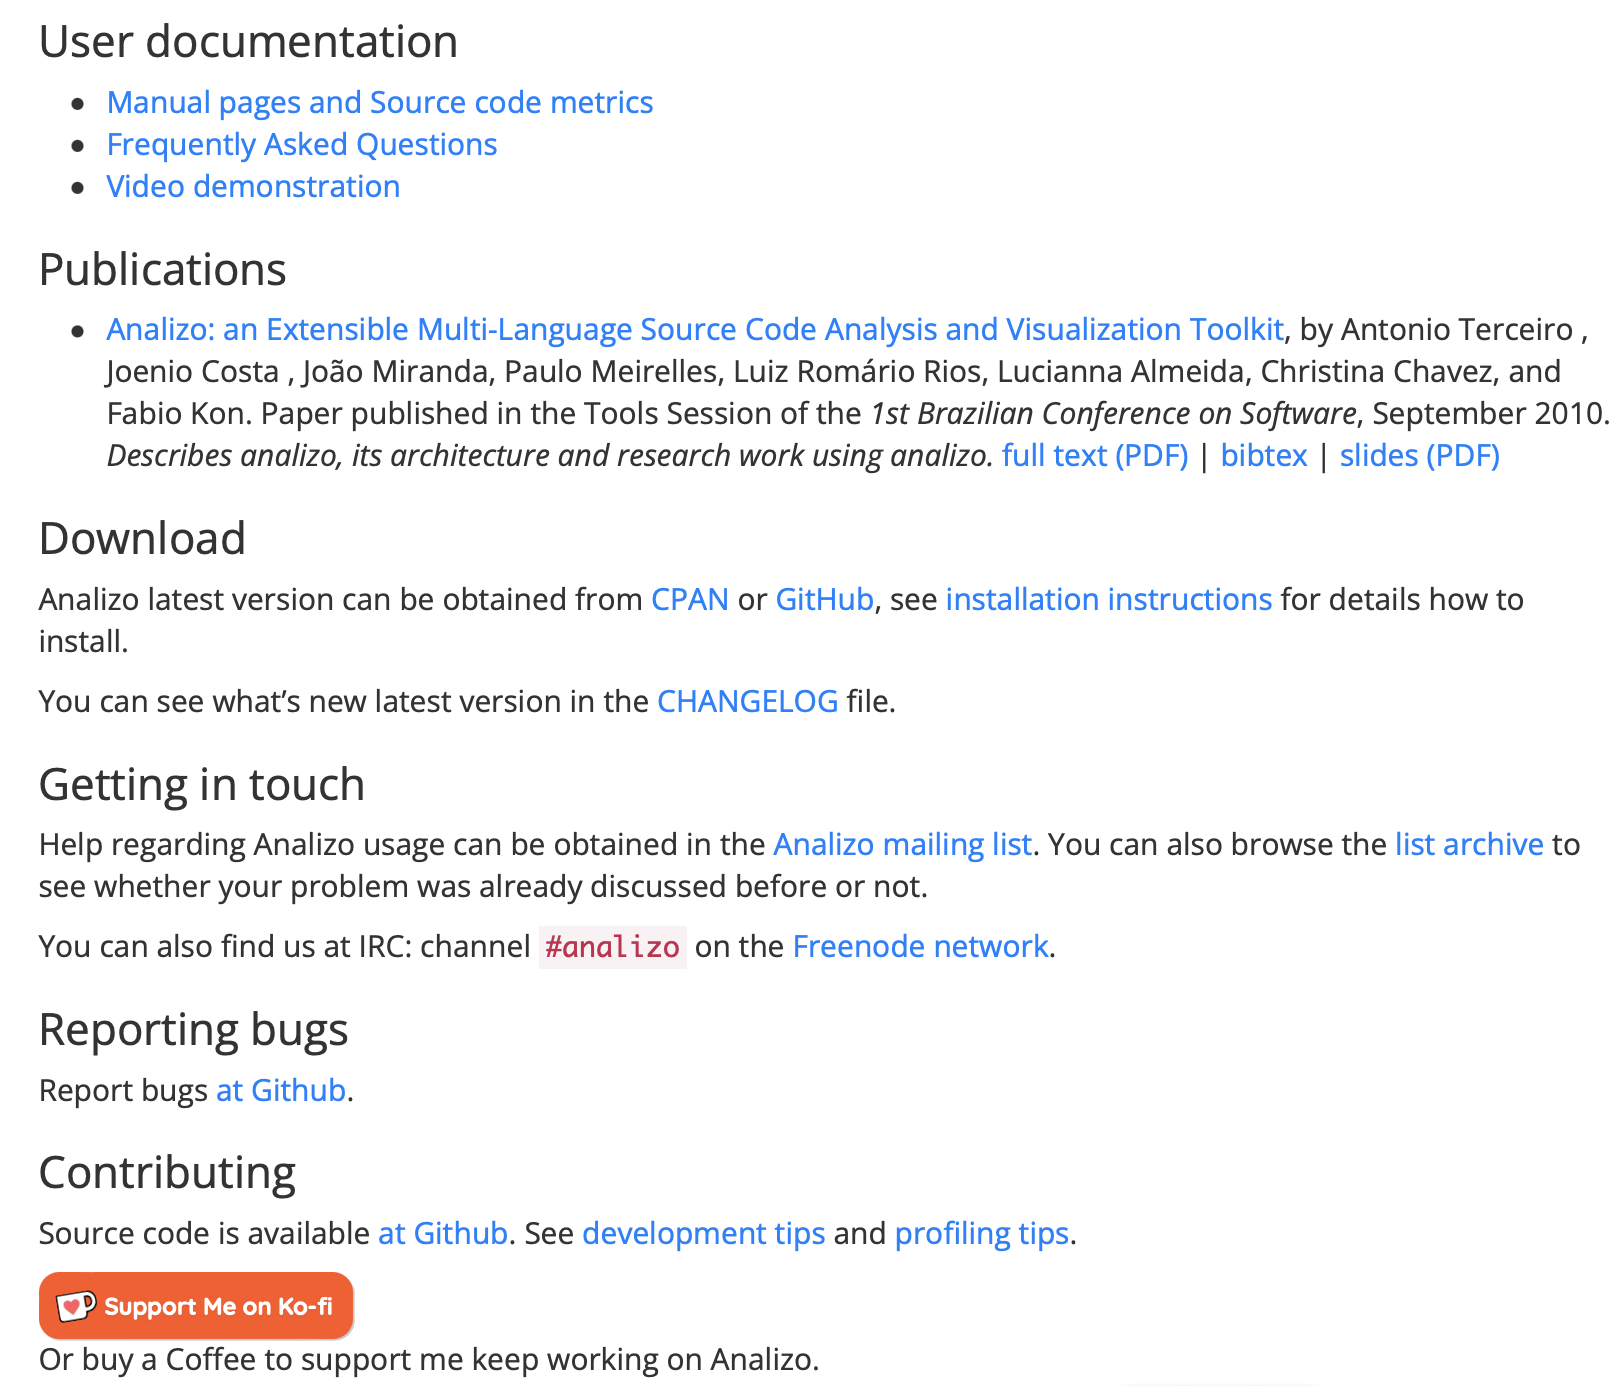
\includegraphics[scale=0.5]{JAI 2023/figures/analizo-website.png}
    \caption{Documentação para usuários da ferramenta \texttt{Analizo}}
    \label{fig:documentacao:analizo}
\end{figure}

%\noindent \textbf{\# \texttt{flossSearch}}.
\noindent \textbf{Exemplo}.
O software \texttt{flosssearch} disponibiliza para os usuários informações sobre funcionalidades, tecnologias e licença utilizada, em um arquivo README, sob controle de versão, que pode ser atualizado regularmente. Porém, não há informações de contato ou sobre canais de comunicação.
A Figura~\ref{fig:documentacao:analizo} mostra uma parte da excelente documentação para usuários disponibilizada no website da ferramenta \texttt{Analizo}\footnote{\url{https://www.analizo.org}}.

%No software \texttt{flosssearch} não há documentação para desenvolvedores com descrição de padrões, ferramentas, fluxos de trabalho, ou testes. 

\subsection{Qualidade}

O processo de garantia da qualidade do \RSw é tão necessário quanto o código que foi escrito.
\textit{Confiabilidade} é um dos atributos de qualidade do software, em geral definido como a probabilidade do mesmo funcionar sem a ocorrência de falhas em um período específico.
Testes e revisão de código são duas técnicas populares que podem ser usadas no desenvolvimento de \RSw confiável.

%----------------------------------%
%Qual a importância dos testes automatizados para o software de pesquisa? 
%Para o software de pesquisa testes podem aumentar a confiabilidade que os resultados produzidos pelo software são mais confiáveis.
%Tipos de testes. testes de unidade e de integração.
%Ferramentas para automação de testes
%------------------------------------%

\subsection*{P8. Teste de software} 

\textit{Teste de software} é a atividade de executar um produto de software para verificar se ele está em conformidade com suas especificações.
Testes fornecem evidências sobre a confiabilidade do software, além de promover agilidade e, possivelmente, redução nos custos de desenvolvimento, depuração e manutenção do software~\cite{maldonado:book}.  

O uso contínuo desta prática protege o \RSw em relação à introdução de \textit{bugs} em correções ou modificações futuras.
%Testes também podem servir para documentar interfaces externas e de funções internas do software.
\textit{Testes de unidade} são usados para testar métodos, funções, \textit{scripts} e outros tipos de unidades de programa, concentrando-se nas saídas geradas em resposta às entradas e às condições de execução~\cite{maldonado:book}. Em geral, os \textit{testes funcionais} tratam o sistema como uma ``caixa preta'', pelo fato de não haver acesso aos detalhes de código para a criação dos casos de teste.

Há diversos \textit{frameworks} disponíveis para criação e \textit{automação de testes} funcionais e de unidade para linguagens de programação popularmente usadas no desenvolvimento de \RS, por exemplo, \textit{JUnit} (http://junit.org/) para Java, \textit{CUnit} (http://cunit.sourceforge.net/) para C, 
\textit{py.test} (http://pytest.org/) para Python e \textit{PHPUnit} (https://phpunit.de) para PHP.

\noindent\textbf{Exemplo.} A ferramenta de análise estática \texttt{Analizo} possui um conjunto de testes automatizados. 
%
A Figura~\ref{fig:testes:analizo} mostra informações sobre como executar seus testes.

%Mostrar um projeto de software de pesquisa que tem testes.
\begin{figure}[tb]
    \centering
    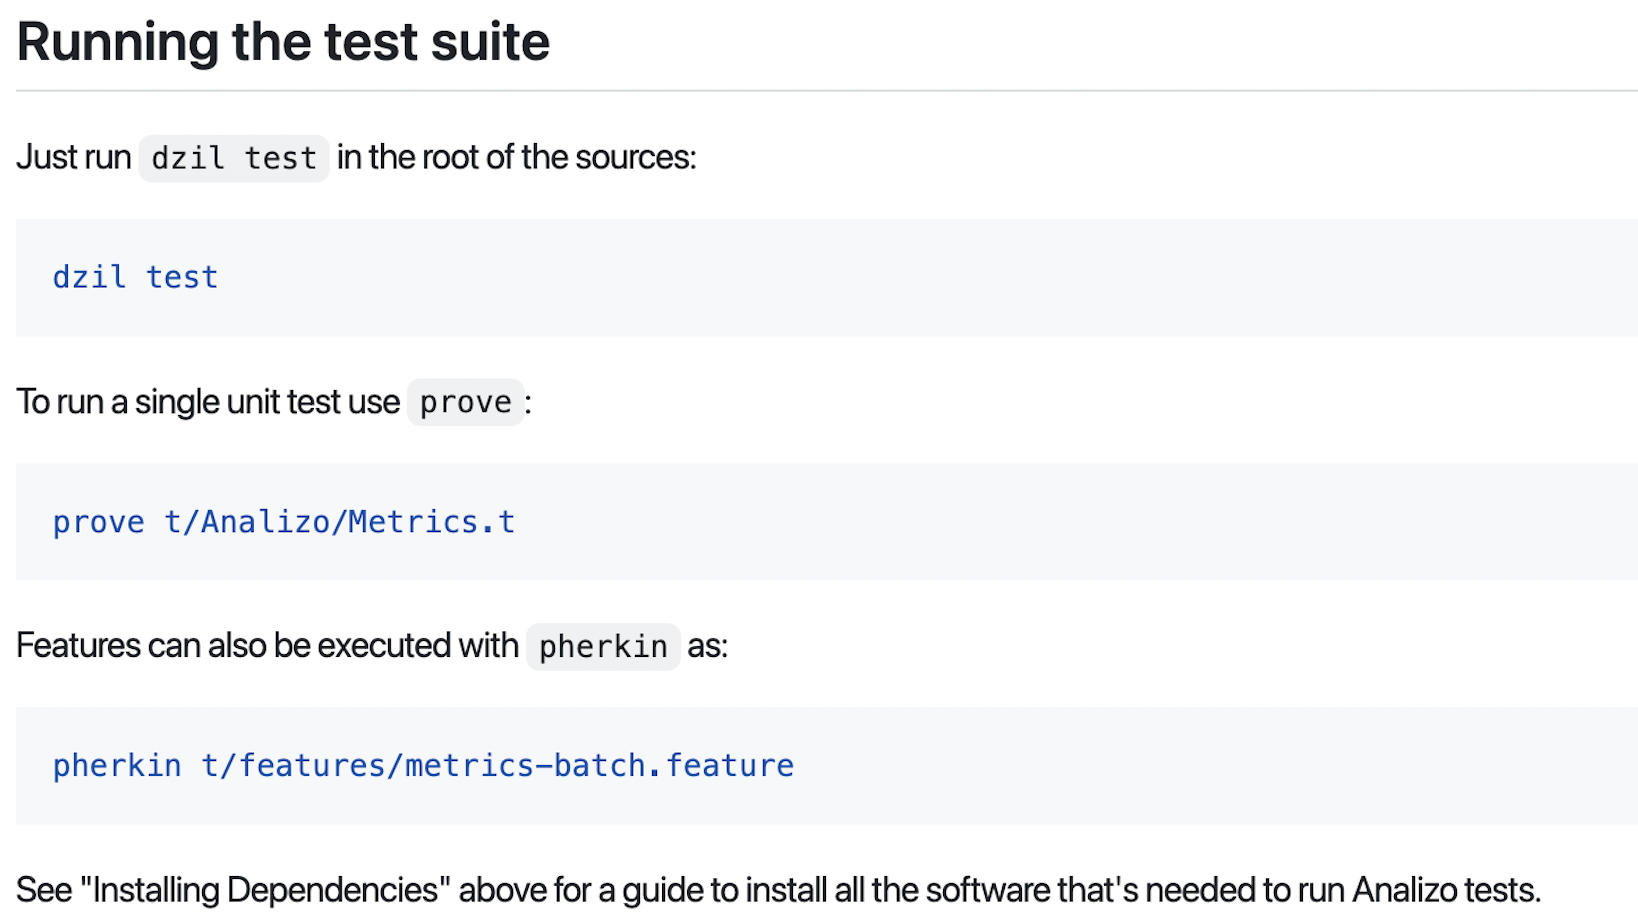
\includegraphics[scale=0.5]{JAI 2023/figures/analizo-tests.png}
    \caption{Trecho da documentação no GitHub mostrando como executar os testes da ferramenta \texttt{Analizo}.}
    \label{fig:testes:analizo}
\end{figure}

Apesar da linguagem PHP possuir um framework para automação de testes, o \textit{PHPUnit}, o software \texttt{flosssearch} não possui testes automatizados. 
A falta de testes pode desestimular os desenvolvedores para consertar, estender ou melhorar o \RS, e desencorajar outros pesquisadores a usá-lo. 

\subsubsection*{P9. Revisão de código} 
% Code reviews are an effective method for improving software quality. 

Revisão de código, ou revisão por pares, é uma prática consolidada para a melhoria da qualidade do software.
A colaboração entre pares durante a revisão é facilitada por meio do acesso compartilhado ao código-fonte e vários canais de comunicação. 
Outros desenvolvedores podem perceber problemas na qualidade do  código do \RSw que testes automatizados podem não detectar. 
Os revisores podem identificar alguns tipos de \textit{bugs}, problemas lógicos, falta de padronização e de conformidade com as práticas e diretrizes do projeto.

No contexto do \RS, a revisão de código pode, além de promover a melhoria da qualidade do software, ser aplicada a outros ativos da pesquisa. 
%
A revisão de código também permite que outros desenvolvedores e pesquisadores avaliem se os métodos aplicados e implementados no \RSw estão em conformidade com as teorias subjacentes da pesquisa. A falta de conformidade entre teoria e implementação em um \RSw  pode levar a conclusões errôneas em todo um estudo e seus resultados.

% Boas práticas na revisão de código.
% Ferramentas.

\noindent \textbf{Exemplo.}
Ao ser colocado em um repositório público, o software 
\texttt{flosssearch} foi compartilhado e pôde ser revisado por outros pesquisadores.
O texto de apresentação mostrado na tela principal do \texttt{flosssearch} em execução, foi revisado por outro pesquisador do grupo e algumas inconsistências foram reportadas e corrigidas.

% Movi pra parte de Avaliação
%\noindent \textbf{\texttt{Software Mosyn}}.
%Por estar publicado no GitHub, é possível fazer \textit{pull requests} e a realização de revisão de código. Até o dia da avaliação, todos os \textit{pull requests} listados no repositórios foram aprovados pelo próprio autor, sugerindo que não houve revisão de código por outra pessoa

\subsection{Gerência}

As práticas de gerência apresentadas estão relacionadas aos processos e ferramentas usados para acompanhar e aumentar a eficiência de tarefas de desenvolvimento do \RS. 

\begin{figure}[tbp]
    \centering
    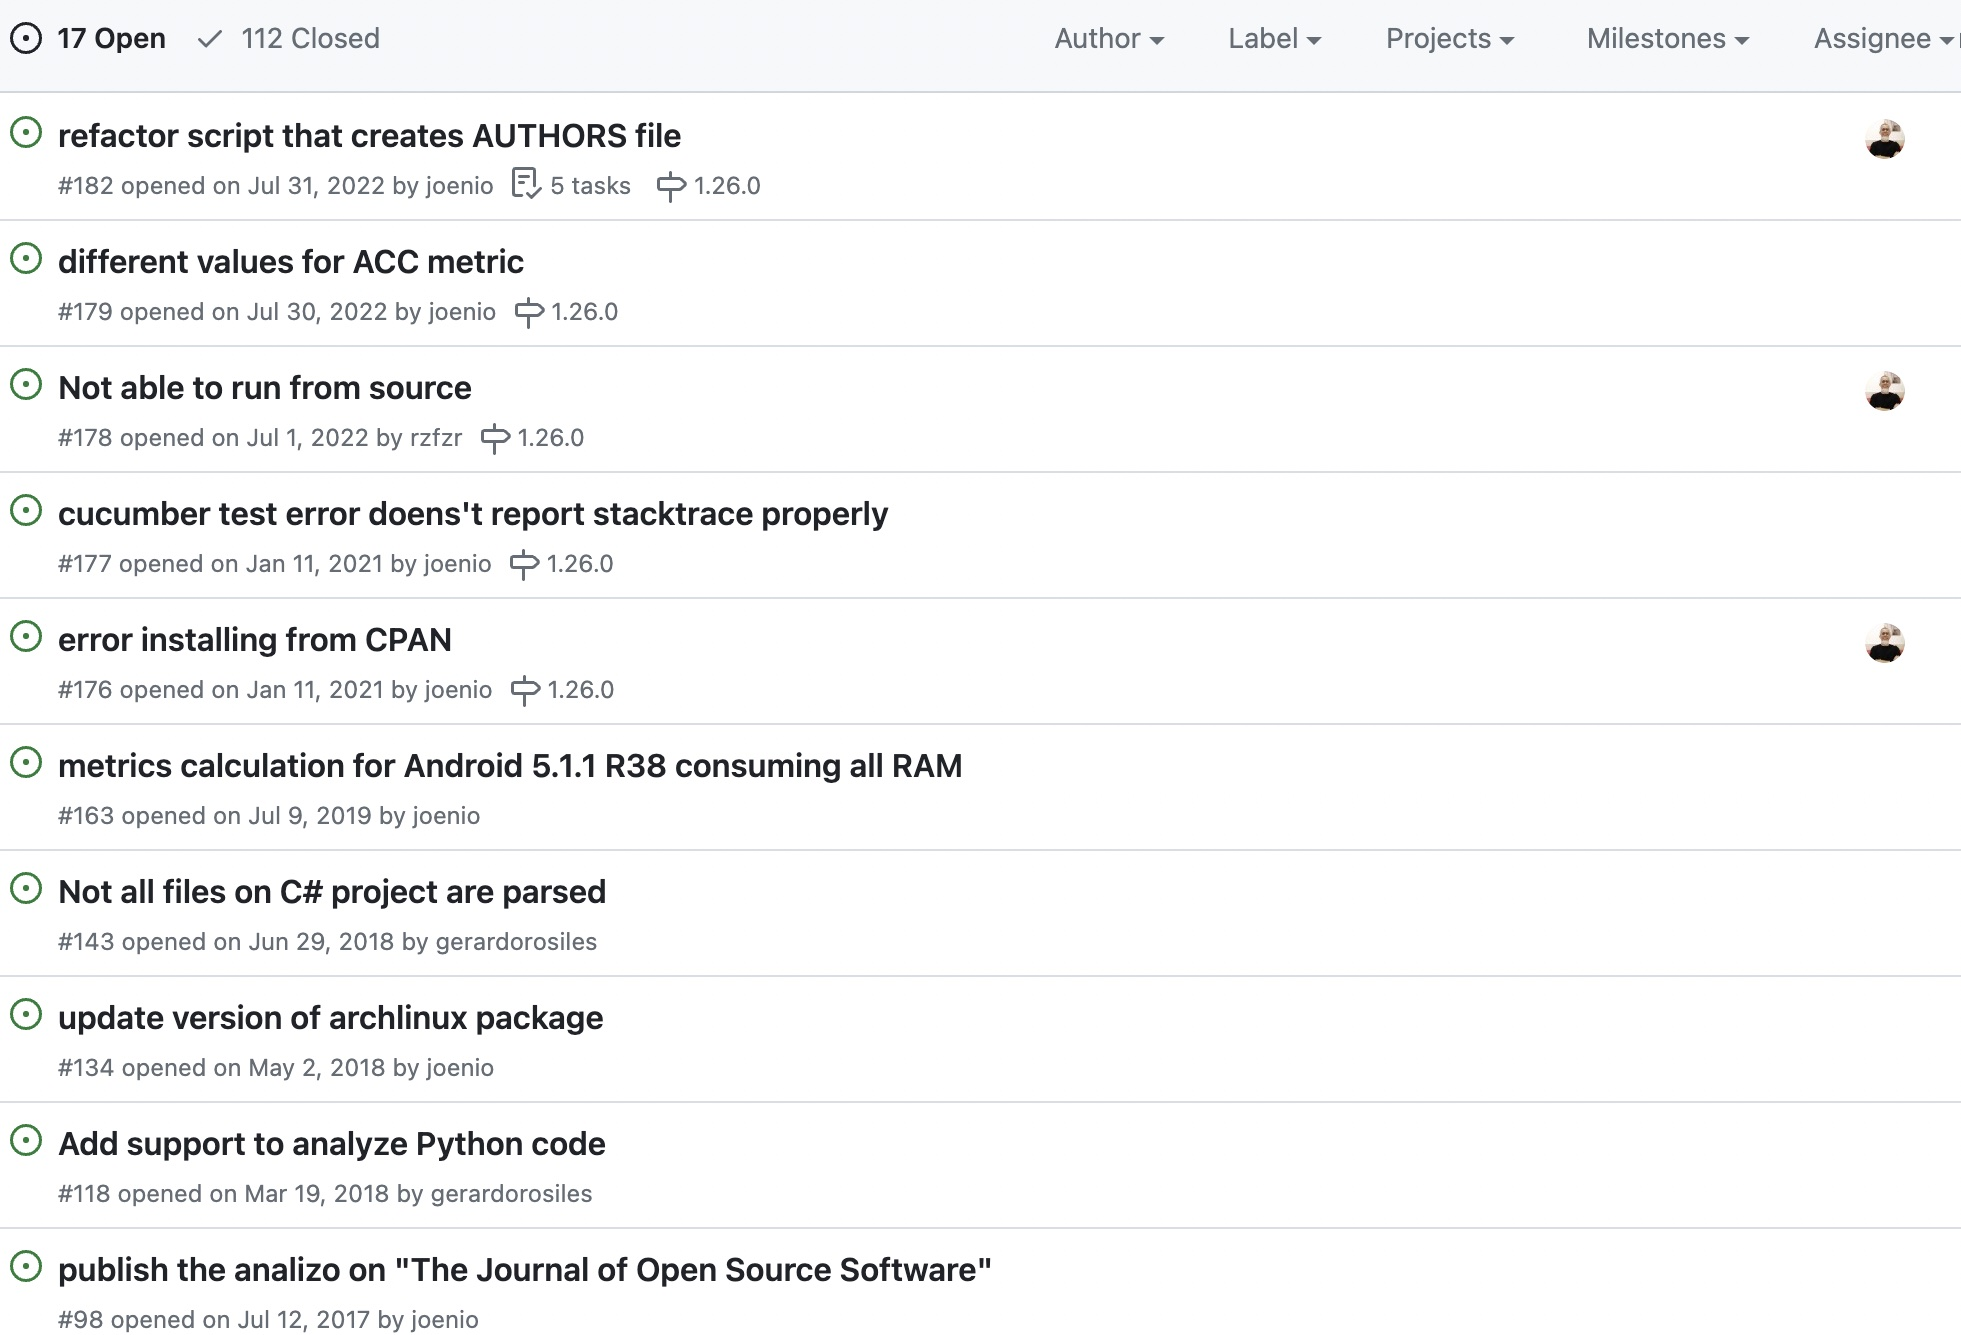
\includegraphics[scale=0.215]{JAI 2023/figures/analizo-issues.jpg}
    \caption{\textit{Issue tracker} da ferramenta \texttt{Analizo} no GitHub.}
    \label{fig:issuetracker:analizo}
\end{figure}

\subsection*{P10. \textit{Issue Trackers} } 

\textit{Issue trackers}\footnote{Usamos o termo em inglês, \textit{issue tracker}, ao invés de traduzí-lo para \textit{rastreador de problemas}, dado que o primeiro é amplamente utilizado pela comunidade internacional de desenvolvedores de software.} 
são ferramentas para rastrear e gerenciar problemas, em geral associados a tarefas como resolução de \textit{bugs} e solicitações de melhoria para um software. 
\textit{Issue trackers} facilitam a colaboração e permitem que os colaboradores acompanhem o progresso das atividades e trabalhem em conjunto para resolvê-las.
Para indicar que o trabalho está em andamento, um desenvolvedor pode vincular uma tarefa (\textit{issue}) 
ao envio de uma solicitação de melhoria no projeto (\textit{pull request}).

% Quais as ferramentas que podem ser utilizadas? 
Em geral, plataformas de hospedagem de repositórios, como Github, Gitlab\footnote{\url{https://gitlab.com}}, Codeberg\footnote{\url{https://codeberg.org}}, e Launchpad\footnote{\url{https://launchpad.net}} oferecem um \textit{issue tracker} nativo e integrado. Alternativas estão disponíveis em ferramentas externas, específicas para gestão de tarefas, dentre elas, Jira, Bugzilla, Trello, e Trac.

No contexto de um \RS, o \textit{issue tracker} também pode ser utilizado para acompanhar a escrita colaborativa de artigos científicos em formato texto simples, usando  linguagens de marcação (\textit{Markdown} ou para \textit{LaTeX}), para posterior processamento.

%Mostrar projeto que usa issue tracker!
\noindent \textbf{Exemplo.}
A Figura~\ref{fig:issuetracker:analizo} apresenta a página do \textit{issue tracker} da ferramenta \textit{Analizo} no GitHub. O projeto recebe solicitações de pessoas externas ao projeto e seus desenvolvedores interagem com os \textit{tickets} criados na tentativa de entender o problema ou ajudar na solução.
%
O software \texttt{flosssearch} não usa o recurso de \textit{issue tracker} do GitHub, nem ferramentas externas com essa finalidade.

\begin{figure}[tbp]
    \centering
    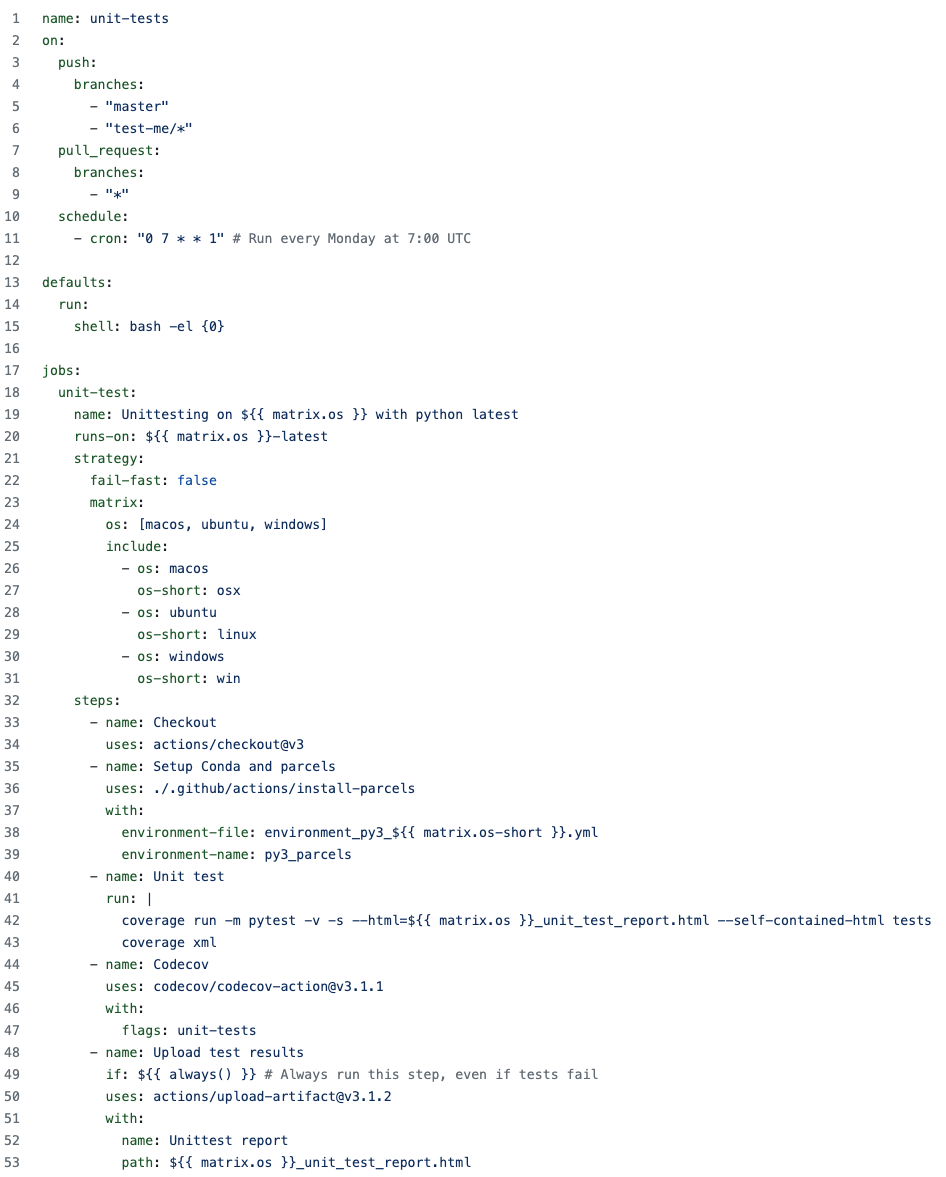
\includegraphics[scale=0.4]{JAI 2023/figures/parcels-automated-tests.png}
    \caption{Fluxo de trabalho automatizados no repositório do \RSw \texttt{Parcels}}
    \label{fig:automatizacao:parcels}
\end{figure}

\subsubsection*{P11. Automatização de tarefas} 

Durante o desenvolvimento de software muitas tarefas são realizadas de forma repetitiva. A automatização permite que essas tarefas sejam executadas de forma rápida e consistente por meio de \textit{scripts}, ferramentas ou sistemas automatizados.
Além dos testes, outras tarefas podem ser automatizadas para ajudar a encontrar e investigar \textit{bugs} mais rapidamente, melhorar a qualidade do software e reduzir o tempo para validação e lançamento de versões do software. 
A automatização pode ser configurada para executar diferentes tipos de testes (unitários, integração), para analisar o código-fonte em busca de problemas de estilo, convenções de codificação ou más práticas, entre outras tarefas. 

\noindent \textbf{Exemplo.}
A Figura~\ref{fig:automatizacao:parcels} mostra um exemplo de automatização de tarefas 
e apresenta um arquivo com a definição de passos para a execução dos testes unitários do \RSw \texttt{Parcels}.

%Ferramentas para analisar a qualidade do código (bugs, erros de estilos, por exemplo).

%Ilustrar com outro software de pesquisa. Sugestão? Colocar figura da tela, mostrando a infra para testes nesse projeto.

%\begin{figure}[htb]
%    \centering
%    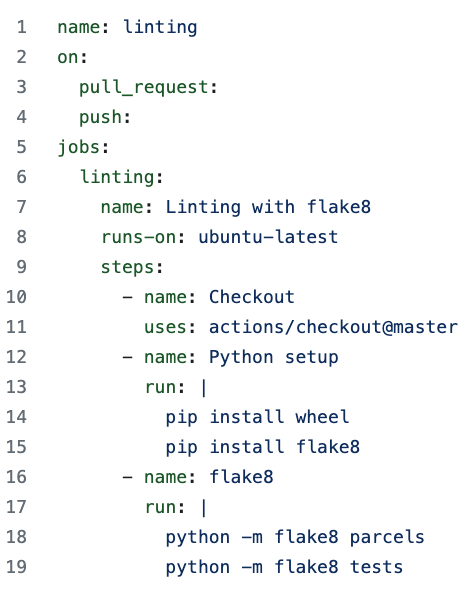
\includegraphics[scale=0.30]{JAI 2023/figures/parcels-automated-lint.png}
%    \caption{Lista de fluxos de trabalho automatizados no repositório do software de pesquisa Parcels}
%    \label{fig:automatizacao:parcels}
%\end{figure}

\subsubsection*{P12. Integração e implantação contínuas} 

\textit{Integração Contínua} (``Continuous Integration'') e \textit{Implantação Contínua} (``Continuous Deployment'') são práticas de automação no desenvolvimento de software que possibilitam a entrega rápida e confiável de um software. 
Na integração contínua, as mudanças são automaticamente verificadas e integradas, permitindo que os problemas sejam detectados e corrigidos mais cedo no processo de desenvolvimento. A implantação contínua permite que as mudanças sejam disponibilizadas automaticamente para os usuários.

%Como utilizar ferramentas de CI/CD no desenvolvimento de
%software de pesquisa?
Para configurar um sistema de integração contínua é necessária a configuração de uma ferramenta, como \textit{Jenkins}, \textit{CircleCI}, \textit{Travis CI} ou \textit{GitHub Actions}, para monitorar o repositório do software e executar automaticamente testes e tarefas de verificação.
A Figura~\ref{fig:ci:cd:parcels} mostra um \textit{pull request} no repositório do \RSw \texttt{Parcels}. 
O projeto implementa integração contínua e, a cada \textit{pull request} nesse repositório, 
tarefas automatizadas são executadas, como testes unitários e de integração e uso de uma ferramenta de análise de código-fonte (\textit{linter}) para identificar possíveis problemas no código. 
Como as tarefas são obrigatórias, o código não poderá ser incorporado ao \textit{branch} principal se alguma das atividades falhar. Na Figura~\ref{fig:ci:cd:parcels}, podemos observar que  os testes unitários falharam.

\begin{figure}[tb]
    \centering
    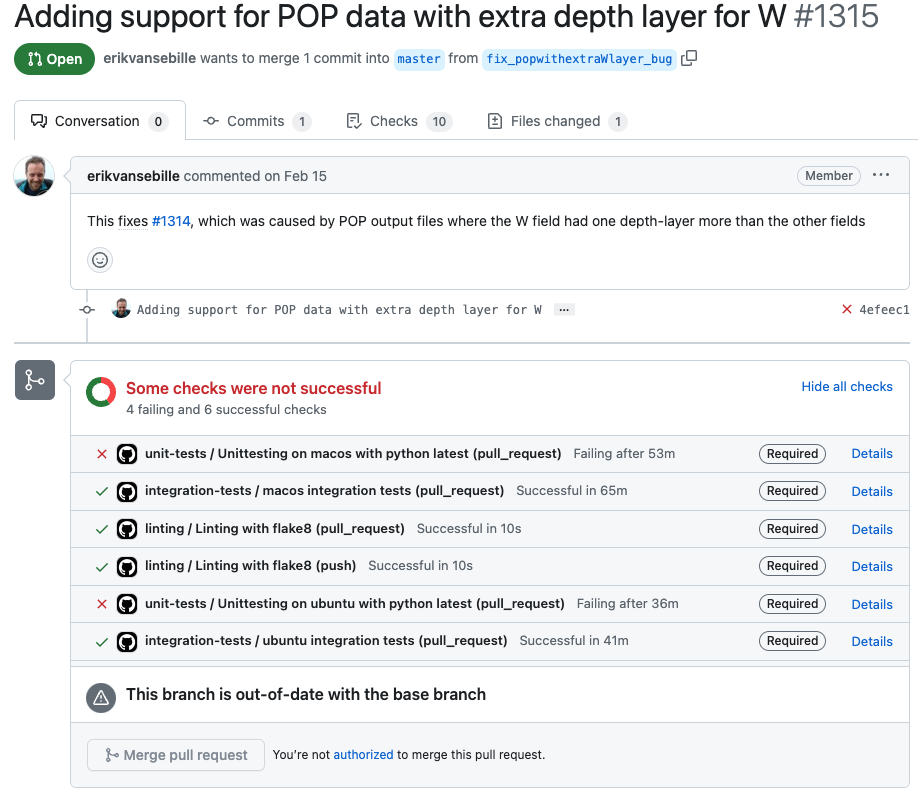
\includegraphics[scale=0.4]{JAI 2023/figures/parcels-pr.png}
    \caption{\textit{Pull request} com testes unitários falhando no repositório do projeto Parcels}
    \label{fig:ci:cd:parcels}
\end{figure}

\begin{figure}[tb]
    \centering
    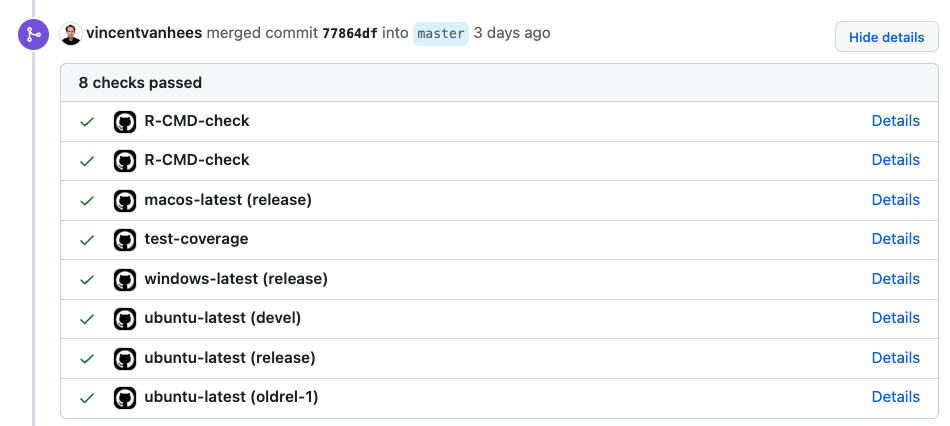
\includegraphics[scale=0.40]{JAI 2023/figures/ggir-ci-cd.png}
    \caption{Tarefas automatizadas executadas após a incorporação de um \textit{pull request} no repositório do \RS.}
    \label{fig:ci:cd:ggir}
\end{figure}

Os \textit{pipelines} de implantação contínua são fluxos de trabalho automatizados que ajudam a \textit{implantar novas versões do software em diferentes ambientes}. Eles podem ser criados usando ferramentas como \textit{Docker}, \textit{Kubernetes}, \textit{GitLab CI/CD} e \textit{CircleCI}.
Para exemplificar a prática, a Figura~\ref{fig:ci:cd:ggir} mostra as tarefas automatizadas realizadas quando um \textit{pull request} é incorporado ao projeto na \textit{branch} principal. O projeto é o \RSw GGIR\footnote{\url{https://github.com/wadpac/GGIR}}, que converte dados brutos de dispositivos vestíveis em relatórios para pesquisadores que investigam a atividade física diária e o sono humano. Após a aprovação do \textit{pull request}, as tarefas automatizadas são executadas e o lançamento da versão.

Ao adotar essas práticas de integração e implantação contínuas no \RS, a confiabilidade do software será maior e a entrega de novas funcionalidades será mais rápida e segura.

%Ilustrar com outro software de pesquisa. Sugestão? Colocar figura da tela, mostrando a infra para CI/CD nesse projeto.

% Movi pra parte de Avaliação
%\noindent \textbf{\texttt{Software Mosyn}}.
%Não há integração contínua. Por ser um plugin instalado manualmente no MATLAB, a implantação contínua não é viável.

\subsubsection*{P13. Lançamento de versões} 

O \textit{lançamento de versões} é importante durante o desenvolvimento de \RSw sustentável para permitir a rastreabilidade das mudanças e permitir que a pesquisa seja reproduzida a partir de uma versão específica do software. O lançamento de versões envolve a marcação de pontos específicos no histórico do código-fonte para representar marcos no desenvolvimento do software. Os repositórios de código fonte fornecem vários recursos que apoiam o lançamento de versões.

Uma estratégia comum é o uso de \textit{tags} (etiquetas), ou marcadores atribuídos a um \textit{commit} para identificar uma versão específica do software. 
As \textit{tags} podem ser usadas para identificar versões estáveis, versões de correção de \textit{bugs}, pontos de lançamento importantes ou algum \textit{milestone} (marco) no desenvolvimento do projeto. Por exemplo, uma \textit{tag} pode ser criada para indicar a primeira versão funcional do software (``versão~1.0'').

Outro recurso importante é o uso de \textit{releases} (lançamentos), com software empacotado e disponibilizado para os usuários. 
\textit{Pacote} (\textit{package}) é o termo utilizado para representar um conjunto organizado de arquivos e recursos relacionados que são distribuídos juntos como uma unidade coesa. O pacote pode incluir o código-fonte do software, dependências, arquivos de configuração, documentação e qualquer outro componente necessário para executar ou instalar o software. A disponibilização do \RSw como pacote facilita a distribuição, instalação e utilização do software, entregando um conjunto funcional de recursos e funcionalidades para os usuários. Cada \textit{release}  pode incluir \textit{release notes} (notas de lançamento) detalhando as alterações, correções de \textit{bugs} e outras informações relevantes.

O nome da versão geralmente segue uma convenção numérica ou alfanumérica, como ``1.0'', ``2.3'' ou também pode incluir um identificador descritivo, como ``versão beta'' ou ``versão alpha''. 
O versionamento semântico\footnote{\url{https://semver.org/lang/pt-BR}} é uma prática comum fortemente recomendável ao adotar e usar versionamento para gerenciar as \textit{releases} do \RS.
%
O \textit{escopo de uma versão} engloba as alterações e atualizações contidas na versão específica, inseridas pelos \textit{commits} incluídos desde a versão imediatamente anterior até a versão sendo lançada. 
Recomenda-se incluir na descrição da \textit{release} informações sobre o seu escopo, por exemplo, funcionalidades adicionadas, problemas resolvidos, melhorias de desempenho, atualizações de segurança e outros detalhes relevantes. Essas informações ajudam a comunicar claramente o que uma determinada versão oferece aos usuários.

\noindent\textbf{Exemplo.}
O \RSw \texttt{Parcels} está em um repositório público e utiliza as funcionalidades de \textit{tags} que descrevem o escopo da versão nos lançamentos de versões.
A Figura~\ref{fig:tags:parcels} apresenta a lista de \textit{tags} no repositório e a Figura~\ref{fig:release:parcels} mostra as notas do lançamento de uma versão do projeto.

\begin{figure}[tbp]
    \centering
    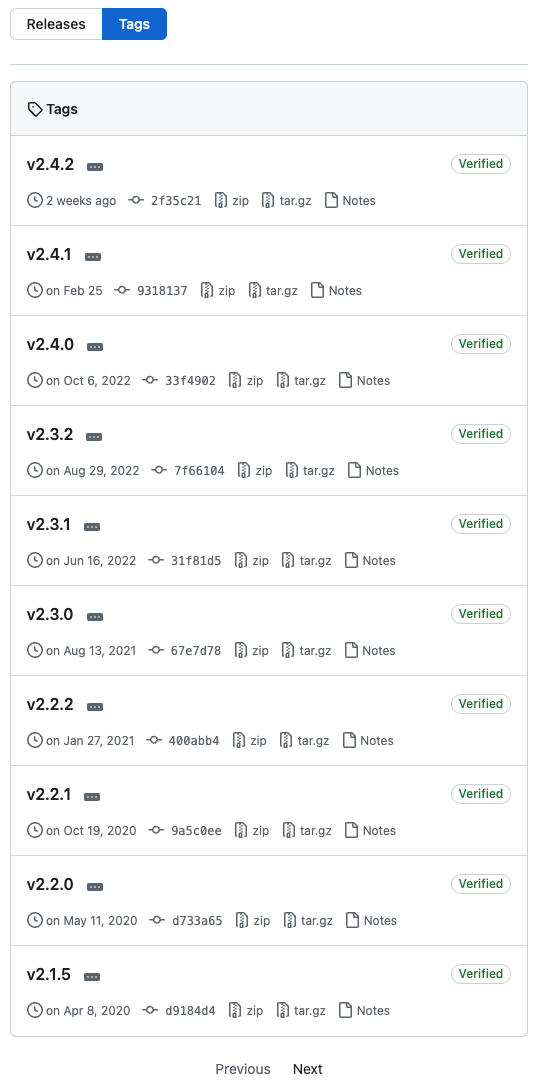
\includegraphics[scale=0.5]{JAI 2023/figures/parcels-tags.png}
    \caption{Lista de \textit{tags} no repositório do software de pesquisa \texttt{Parcels}.}
    \label{fig:tags:parcels}
\end{figure}

\begin{figure}[tbp]
    \centering
    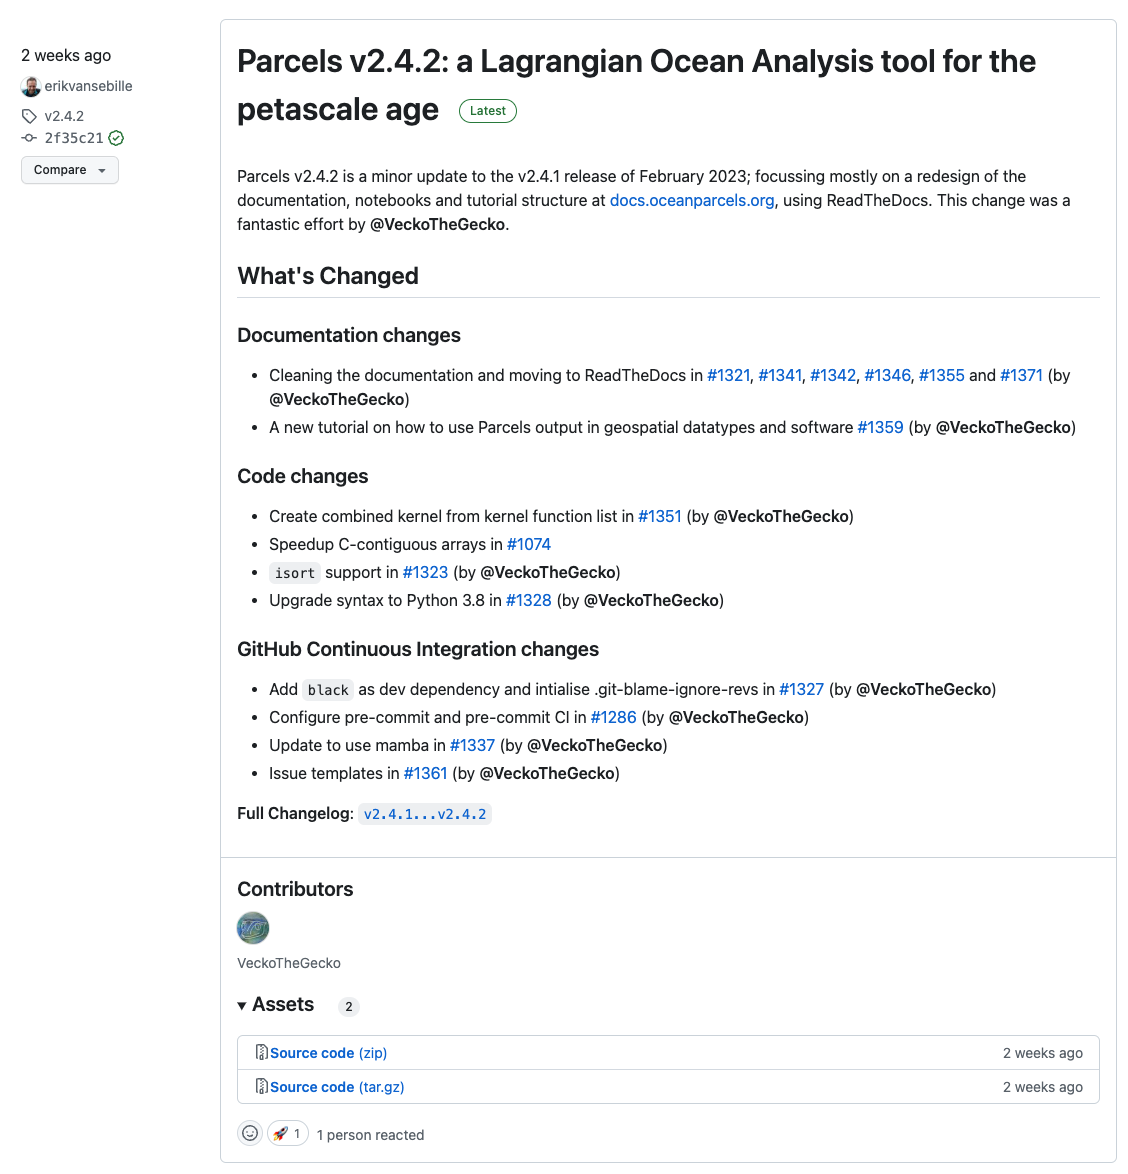
\includegraphics[scale=0.40]{JAI 2023/figures/parcels-release.png}
    \caption{Notas de lançamento de uma versão no repositório do software de pesquisa Parcels.}
    \label{fig:release:parcels}
\end{figure}

%------------------------------------%

\begin{comment}
\subsection{Aspectos de Comunidade}
%“I have my first pull request, and the beginning of a community. What now?” Returns in more depth to issues of licensing and release management, with added information about community-building and sustainability concerns.

\textit{Quero usuários:} Release your software; Provide user documentation; Easy installation; Provide issue tracker.

\textit{Quero contribuidores:} 
Provide development documentation; Provide a means of communication; Implement and add a code of conduct; 
Contribution guideline.

%\textit{Quero reconhecimento:} forma de citar software ...
\end{comment}

%------------------------------------%
\subsection{Reconhecimento}

As boas práticas que promovem a sustentabilidade técnica do \RSw podem atrair usuários e contribuidores para o software.
%
As práticas apresentadas a seguir estão relacionadas com o reconhecimento da relevância do \RSw para outros pesquisadores e da necessidade de sua divulgação e citação apropriadas.

\subsubsection*{P14. Comunidade do projeto} 

Em geral, o \RSw é desenvolvido por indivíduos ou em pequenos grupos de pesquisa dentro de uma única instituição, resultando em protótipos para atender às suas próprias necessidades, por exemplo, validar uma hipótese ou apoiar atividades da pesquisa.
%
Criar uma comunidade em torno de um \RSw é essencial para aumentar a adoção e colaboração, ampliando seu impacto na comunidade científica. 
Além disso, a comunidade ajuda na identificação e correção de problemas e traz novas sugestões para o desenvolvimento do software. 

Uma comunidade ativa e engajada promove a colaboração entre pesquisadores e desenvolvedores de diferentes instituições e áreas de pesquisa. Tal engajamento facilita a troca de ideias, a discussão de problemas, a identificação de \textit{bugs}, a proposição de novas funcionalidades, a implementação de melhorias e novas funcionalidades para o software. 
Outra vantagem da comunidade é realizar revisão por pares do código-fonte, documentação e resultados produzidos pelo software. Essas revisões ajudam a garantir a qualidade e a confiabilidade do software. A diversidade de perspectivas e experiências na comunidade contribui para um processo de desenvolvimento mais completo. Além disso, a existência de uma comunidade ativa em torno do \RSw pode aumentar sua sustentabilidade no longo prazo. 
Com uma base de usuários e desenvolvedores engajados, o software tem maior probabilidade de receber suporte financeiro, recursos e atualizações contínuas, facilitando sua disponibilidade e relevância para outros pesquisadores.

%- Estratégias para envolver usuários e colaboradores, estabelecer diretrizes para participação, reconhecer e valorizar as contribuições e \textit{manter canais de comunicação, como fóruns de discussão, listas de e-mails, chat e eventos}.

Para envolver usuários e colaboradores em um \RS, é importante estabelecer diretrizes claras, reconhecer e valorizar as contribuições, disponibilizar canais de comunicação, organizar eventos e atividades, fornecer documentação detalhada e acessível e incentivar a colaboração ativa.

%É mais provável que os usuários e colaboradores se sintam encorajados a participar se o projeto estabelecer 
As diretrizes que orientam a participação na comunidade abordam aspectos sobre como contribuir com código, como reportar problemas e participar em discussões. Idealmente, o projeto deve disponibilizar um código de conduta e um guia sobre como contribuir.
Quando definidas e seguidas, diretrizes ajudam a criar um ambiente colaborativo e respeitoso. 
%
Outra estratégia essencial é reconhecer e valorizar as contribuições dos usuários e colaboradores. Com agradecimentos públicos, inclusão de nomes nos créditos do projeto, menções em publicações relacionadas ao \RSw e outros gestos de reconhecimento, incentivam-se o engajamento contínuo e a motivação para continuar colaborando com o projeto.

Para facilitar a interação entre os membros da comunidade é fundamental disponibilizar \textit{canais de comunicação}, como fóruns de discussão online, listas de e-mails, salas de bate-papo e plataformas como GitHub e GitLab. 
Esses canais permitem que os colaboradores obtenham suporte técnico, compartilhem ideias, troquem experiências e contribuam com melhorias no \RS. Também é possível promover a interação direta entre os membros da comunidade com a organização ou participação em conferências, workshops, treinamentos e eventos.

Para incentivar a colaboração ativa dos usuários é importante a identificação de tarefas específicas que precisam de contribuições, a criação de programas de mentoria para novos colaboradores, orientações claras sobre como contribuir para o projeto. 
Por fim, é essencial fornecer uma documentação detalhada e acessível para que os colaboradores possam compreender e utilizar o software de forma eficaz. 

%\textbf{Suporte para reprodutibilidade?}

%\textit{Quero contribuidores:} Provide development documentation; Provide a means of communication; Implement and add a code of conduct; Contribution guideline.

\noindent\textbf{Exemplo.} 
% Um artigo de Terceiro da época do doutorado?
A ferramenta \texttt{flosssearch} foi implementada em PHP, por conveniência e experiência do desenvolvedor, pensando na construção de uma comunidade que, no futuro, poderia transformar \texttt{flosssearch} em um produto.
Porém não há políticas ou recomendações definidas para os membros da comunidade.
% Movi pra parte de Avaliação
%\noindent \textbf{\texttt{Software Mosyn}}.
%Apenas o usuário dono do repositório submeteu \textit{commits} e \textit{pull requests} no projeto. A página do projeto não apresenta outros usuários que adicionaram o projeto como favorito e não mostra usuários que fizeram uma cópia (\textit{fork}) independente do projeto.

A plataforma GitHub apresenta suas políticas e recomendações para os membros da comunidade\footnote{\url{https://docs.github.com/en/site-policy/github-terms/github-community-guidelines}}, incentivando-os a
moderar seus projetos sempre que possível e denunciar qualquer conteúdo que possa violar tais políticas.

\subsubsection*{P15. Divulgação de Software} 

%Divulgação em eventos científicos, estudos com outros pesquisadores para avaliar usabilidade da ferramenta e potencial interesse.

A divulgação do \RSw em eventos científicos e estudos com outros pesquisadores é de extrema importância. Essas oportunidades permitem que os pesquisadores compartilhem e apresentem suas soluções de software, que avaliem a usabilidade da ferramenta e potenciais interesses em comum.
 
Ao apresentar o \RSw para a comunidade acadêmica e colaborar com outros pesquisadores, é possível receber opiniões, estabelecer parcerias, trocar conhecimento e, talvez, aumentar o impacto e a adoção do software de pesquisa, impulsionando o alcance da ciência.

%Quando o \RSw for usado em artigos científicos, é preciso registrar qual a versão do software foi utilizada em cada artigo.
% Um artigo de Terceiro da época do doutorado?
\noindent \textbf{Exemplo.}
O software \texttt{flosssearch} foi utilizado e publicado em artigos científicos, tanto como instrumento da pesquisa, como produto da pesquisa. Entretanto, ainda não há informações  documentadas no repositório sobre a correspondência entre artigos publicados e versões do software.

O arquivo README do \texttt{Parcels} apresenta uma seção sobre ``manuscrito e código'', onde cita artigos publicados e a versão software usada:
\begin{quote}
The manuscript detailing the performance of \texttt{Parcels v2.4} is available at Computers \& Geosciences and can be cited as:

Kehl, C, PD Nooteboom, MLA Kaandorp and E van Sebille (2023).
\textit{Efficiently simulating Lagrangian particles in large-scale ocean flows -- Data structures and their impact on geophysical applications}, Computers and Geosciences, 175, 105322. 
https://doi.org/10.1016/j.cageo.2023.105322
\end{quote}

\subsubsection*{P16. Citação de Software} 

%Citação de \textit{Research Software} para que pesquisadores e desenvolvedores recebam crédito por seu trabalho.
A boa prática científica exige que o \RSw mencionado em publicações científicas seja mantido para reprodutibilidade e verificação de resultados científicos.
%
Citar um software de pesquisa é uma forma de reconhecer e dar visibilidade aos autores e ao próprio software, possibilitando que outros pesquisadores o localizem e eventualmente reusem. Entretanto, 
a citação de software em publicações científicas ainda não é uma prática comum entre cientistas, mas padrões de citação têm sido propostos e adotados. 

Em seu artigo ``Recognizing the value of software: a software citation guide'',  \cite{katz:citation:format} apresentam instruções simples sobre como o software pode se tornar citável e destacam que o uso de identificadores persistentes (PIDs) e metadados descritivos são elementos essenciais da citação de software. 
Informações sobre autoria, nome, local de publicação, data de publicação e identificador do software são consideradas obrigatórias.
%
Adicionalmente, alguns estilos de citação pedem uma descrição da citação entre colchetes. Para software, pode-se usar \textit{[Computer software]}.
A Tabela~\ref{tab:citation:format} apresenta o formato de citação de software proposto por~\cite{katz:citation:format}.

\begin{table}[htb]
    \centering
        \caption{Formato de Citação de Software \cite{katz:citation:format}.}
    \label{tab:citation:format}
    \begin{tabular}{p{2.5cm}|p{11.5cm}}
    \hline
        \textbf{Informação} & \textbf{Descrição} \\
    \hline
        \textbf{Criador(es)} & Autor(es) ou projeto que desenvolveram o software \\
        \textbf{Título} & Nome do software \\
        \textbf{Local} & Local de publicação do software, por exemplo, um arquivo ou repositório que fornece identificadores persistentes. \\
        \textbf{Data} & Data em que o software foi publicado, por exemplo, a data associada a um lançamento ou versão do software.\\
        \textbf{Identificador} &  Um apontador resolvível para o software,  de preferência um PID que leve para uma página contendo metadados descritivos sobre o software, semelhante a um DOI. \\
    \hline
    \end{tabular}
\end{table}

%What is a CITATION.cff file?
%Citation File Format (CFF) (Druskat et al. 2021) (v1.2.0) are plain text files with human- and machine-readable citation information for software (and datasets). Code developers can include them in their repositories to let others know how to correctly cite their software.
%This format is becoming popular within the software citation ecosystem. Recently GitHub, Zenodo and Zotero have included full support of this citation format (Druskat 2021). GitHub support is of special interest:

%
O formato \textit{Citation File Format} (CFF)\footnote{\url{https://citation-file-format.github.io}} tem se popularizado como formato e padrão para documentar como citar um projeto de software~\cite{druskat:2021}.
%
Adicionar um arquivo {\em CITATION.cff} ao repositório do \RSw pode ser uma boa forma documentar e atualizar as recomendações definidas para citação do software. 
Recentemente, Zenodo e GitHub facilitaram a adição de metadados aos repositórios e a geração de citações para esses 
repositórios~\cite{smith:2021}. 

Além disso, pode-se definir um ID persistente para o \RS, por exemplo, um DOI obtido para um artigo que apresenta o software para a comunidade (\textit{software paper}) ou ainda usar formatos mais recentes como o SWHID\footnote{\url{https://www.swhid.org}} promovido pelo projeto Software Heritage\footnote{\url{https://www.softwareheritage.org}}, uma iniciativa dedicada a coletar e preservar software em formato de código-fonte para preservação e acesso público.
%
Entretanto, \cite{katz:citation:format} recomendam que, se existir um artigo que apresenta o \RSw para a comunidade científica, ele deve ser citado como uma referência bibliográfica \textit{adicional}, mas não deve substituir a citação do software propriamente dita.

\noindent\textbf{Exemplo.} 
O \RSw \texttt{flosssearch} não definiu como deve ser citado. 
A ferramenta \texttt{Analizo} indica uma publicação que pode ser considerada como citação para o software~\cite{analizo2010} mas não apresenta uma citação de software.

%Ele foi usado em cinco estudos nos últimos quatro anos, porém os artigos científicos mencionam apenas a sua URL, sem detalhes sobre a versão utilizada. 

\begin{comment}

\begin{table}[htb]
\begin{tcolorbox}[colback=white,title=Descrição do Software de Pesquisa]
\begin{description}
    \item [\texttt{flosssearch.}] Software para apoio à busca e seleção de um projeto OSS para uso na Educação em Engenharia de Software.
    \item[Funcionalidades.] xxx.
    \item[Linguagem de programação.] PHP 5.6 (99.3\%)
    \item[Citação.] M. Brito, B. Lessa, C. Flach. "flossearch".
    \item[Versão.] 1.0
    \item[Licença.] GPL 3.0
    \item[URL.] ...
\end{description}
\end{tcolorbox}
\end{table}
   
\end{comment}


% Para software, essas mudanças incluem a publicação de artigos sobre software, tanto em periódicos gerais quanto em periódicos especializados em artigos sobre software (por exemplo, Journal of Open Source Software Smith et al., 2018), bem como chamadas para citação direta de software ( Smith et al., 2016) juntamente com orientações para essas citações (Katz et al., 2021). 
% O software, como um objeto digital, também tem a vantagem de ser geralmente armazenado como uma coleção de arquivos, muitas vezes em um repositório de software. Esse fato significa que é relativamente simples adicionar um arquivo adicional contendo metadados sobre o software, incluindo criadores e contribuições, em um dos vários estilos possíveis (Wilson, 2013; Druskat, 2020; Jones et al., 2017). 
% O GitHub recentemente reforçou esse esforço, o que facilitou a adição desses metadados aos repositórios e a geração de citações para esses repositórios (Smith, 2021).

